\chapter{Pictorial structures: \\Pose estimation meets structured prediction} 
\label{sec:ps}
Classical pictorial structure models (PS models) are a class of structured 
models specifically proposed to represent 2D objects with parts which can 
articulate in a kinematically plausible way.  The model was first proposed by 
\citet{fischler1973ps}, and has been hugely popular in computer vision since 
computational innovations by \citet{felz05}.

Pictorial structures take the form of a pairwise structured model as described 
in \secref{pairwise-mrf}:
\begin{equation}
s(x,y) = \sum_{i \in \cV_G} \phi_i(x,y_i) + \sum_{ij \in \cE_G} 
\label{eq:standard-ps}
\phi_{ij}(y_i-y_j)
\end{equation}
with the important exception that {\em the pairwise terms $\phi_{ij}(y_i-y_j)$ 
are image-independent}---they are not a function of $x$.

In PS models, the variables correspond to the major body parts.  For upper-body 
pose estimation, $y$ typically corresponds to \{head, torso, left upper arm, 
left lower arm, right upper arm, right lower arm\}, and $y_i \in 
\{1,2,3,\ldots,80\times 80 \times 24\}$ represents a typical $80 \times 80$ 
discretized grid of spatial locations, and $24$ discretized angles for each 
part.  Thus one way to think about the representation for each part is a unit 
vector describing position and orientation of each limb, and the state space as 
a 3D cuboid. 

\mypar{Edge structure:} In order to support tractable inference, the part 
interaction structure $G$ must be a tree (\secref{inference}).  The most common 
tree is formed by considering kinematic connections only: the lower-arm is 
connected to the upper-arm, the upper-arm to the torso, etcetera.

\mypar{Unary potentials:} The unary potentials $\phi_i(x,y_i)$ encode how 
likely a limb is at location/orientation $y_i$ in the image.  This can be 
thought of as a part detector applied to an image patch located at $y_i$.  In 
practice these detectors are patch-based sliding window object detectors, 
applied at every location and orientation.  The typical representation is based 
on edge information in order to be invariant to lighting and color. Edge 
orientation and magnitude are often locally quantized and histogrammed to be 
more numerically and spatially stable, and invariant to local signal gain.  
Feature representations are discussed in detail in \secref{features}.

\mypar{Pairwise potentials:} Pictorial structures assumes a restricted form of 
pairwise potential the depends only on the deformation between kinematially 
attached parts. In general, this is a quadratic stretching cost of the form 
\begin{align} \label{eq:springcost}
\phi_{ij}(y_i-y_j) = -||T_{ij} y_i - T_{ji} y_j - \delta_{ij} ||_2^2 
\end{align}
where $T_{ij}$ are rigid transformations (rotation, translation and scale) to 
place neighboring parts in a local coordinate frame, and $\delta_{ij}$ is the 
expected displacement between the parts.  For example, 
$\phi_{ij}(y_{\text{luarm}} - y_{\text{llarm}})$ measures the squared Euclidean 
distance between the elbow locations according to the left upper arm and left 
lower arm variables.  

\mypar{Spring model interpretation} The reasons for restricting the pairwise 
potential to be only a function of spatial deformation are primarily 
computational, as discussed in \secref{dt}.  In addition, this type of model is 
simple and intuitive to interpret as a ``spring model'' of object layout: the 
PS model can be interpreted as a set of springs at rest in default positions 
$\delta_{ij}$ stretched by displacement $T_{ij} y_i - T_{ji}y_j $.  The spring 
tightness is encoded by warping transformations $T_{ij}$ which can scale the 
dimensions of the spatial Euclidean coordinate space.  The unary terms pull the 
spring ends towards locations $y_i$ with higher scores $\phi_i$ which are more 
likely to be a location for part $i$.  Thus the spring model seeks a balance 
between confidence in individual part detectors, and the amount of deformation 
from a default, 2D geometric prior of the human layout.  \figref{spring-model} 
provides an illustration.

\begin{figure}[tb]
\begin{center}
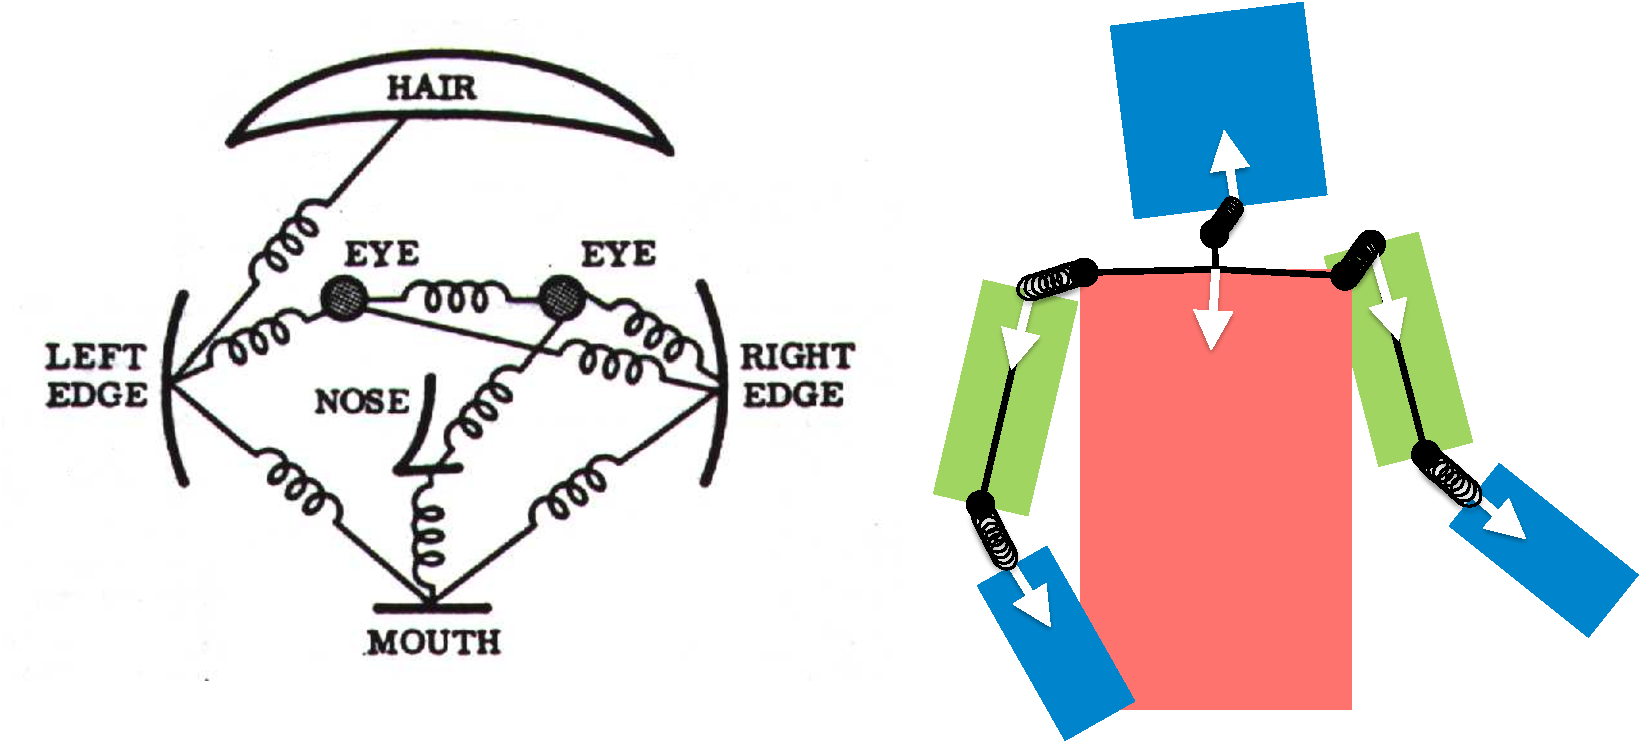
\includegraphics[width=0.99\textwidth]{figs/spring-model.pdf}
\caption[Spring model of pose.]{Spring model of pose.  At left, the original 
spring pictorial structure model that appeared in \citet{fischler1973ps}. At 
right, the standard PS model for 2D human pose.  The states are shown as unit 
vectors indicating the position of joints and their direction.  The mean 
displacement between joints are shown as solid black circles, connected by 
solid black lines to show the kinematic tree structure.  The displacement from 
mean positions are shown as springs stretching.}
\label{fig:spring-model}
\end{center}
\end{figure}

\out{
spring model
geometric or structural prior
loose-limbed


 to models where the nodes of the graph represents object parts, and edges 
between parts encode pairwise geometric relationships.  For modeling human 
pose, the standard PS model decomposes as a tree structure into unary 
potentials (also referred to as appearance terms) and pairwise terms between 
pairs of physically connected parts.  Figure~\ref{fig:ps} shows a PS model for 
6 upper body parts, with lower arms connected to upper arms, and upper arms and 
head connected to torso.  In previous 
work~\cite{devacrf,felz05,ferrari08,posesearch,andriluka09}, the pairwise terms 
do not depend on data and are hence referred to as a spatial or structural 
prior.
%\begin{figure}[]
%\begin{center}
%\centerline{\includegraphics[width=0.75\columnwidth]{data/model_parameters2.pdf}}
%\caption{Basic upper-body model with part state $l$ and part support rectangle of size $(w,h)$.}
%\label{fig:ps}
%\end{center}
%% \vskip -0.5in
%\end{figure}
The state of part $i$, denoted as $y_i \in \mathcal{Y}_i$, encodes the joint 
location of the part in image coordinates and the direction of the limb as a 
unit vector: $y_i = [y_{ix} \; y_{iy} \; y_{iu} \; y_{iv}]^T$. The state of the 
model is the collection of states of $M$ parts: $p(ys = ys) = p(y_1 = y_1, 
\ldots, y_M = y_M)$.  The size of the state space for each part, 
$|\mathcal{Y}_i|$, the number of possible locations in the image times the 
number of pre-defined discretized angles. For example, standard PS 
implementations typically model the state space of each part in a roughly $100 
\times 100$ grid for $y_{ix} \times y_{iy}$, with 24 different possible values 
of angles, yielding $|\mathcal{Y}_i| = 100 \times 100 \times 24 = 240,000$. The 
standard PS formulation (see~\cite{felz05}) is usually written in a 
log-quadratic form:
\begin{align}
p( ys | x) &\propto \prod_{ij} \exp(-\frac{1}{2}||\Sigma_{ij}^{-1/2}(T_{ij}(y_i) - y_j - \mu_{ij})||_2^2)  \times \prod_{i=1}^M \exp(\mu_i^T\phi_i(y_i,x))
\label{eq:standard-ps}
\end{align}
The parameters of the model are $\mu_i,\mu_{ij}$ and $\Sigma_{ij}$, and 
$\phi_i(y_i,x)$ are features of the (image) data $x$ at location/angle $y_i$.  
The affine mapping $T_{ij}$ transforms the part coordinates into a relative 
reference frame.  The PS model can be interpreted as a set of springs at rest 
in default positions $\mu_{ij}$, and stretched according to tightness 
$\Sigma^{-1}_{ij}$ and displacement $\phi_{ij}(ys) = T_{ij}(y_i) - y_j$.  The 
unary terms pull the springs toward locations $y_i$ with higher scores 
$\mu_i^T\phi_i(y_i,x)$ which are more likely to be a location for part $i$.

This form of the pairwise potentials allows inference to be performed faster than $O(|\mathcal{Y}_i|^2)$:  MAP estimates $\argmax_{ys} p(ys | x)$ can be computed efficiently using a generalized distance transform for max-product message passing in $O(|\mathcal{Y}_i|)$ time.  Marginals of the distribution, $p(y_i | x)$, can be computed efficiently using FFT convolution for sum-product message passing in $O(|\mathcal{Y}_i| \log |\mathcal{Y}_i|)$~\cite{felz05}.

While fast to compute and intuitive from a spring-model perspective, this model has two significant limitations.  One, the pairwise costs are unimodal Gaussians, which cannot capture the true multimodal interactions between pairs of body parts.  Two, the pairwise terms are only a function of the geometry of the state configuration, and are oblivious to the image cues, for example, appearance similarity or contour continuity of the a pair of parts.
}

\section{Sub-quadratic inference}\label{sec:dt}

As discussed in \secref{pairwise-mrf}, the computation required to obtain the 
highest-scoring pose out of the exponentially-many possibilities according to 
\equref{standard-ps} is $O(kn^2)$, using \algref{max-inference}.  In pose 
estimation, the reason is intuitive: for each possible location of, say a left 
upper arm, we need to exhaustively search to find the best location of a 
corresponding lower arm, checking all such possibilities of left lower arms.  
Doing this for all left upper arms yields an exact $n^2$ search.

In practice, there is no need to check {\em all} possibilities of lower arms 
for each upper arm location; it is sufficient to check only in a reasonable 
spatial window around the mean displacement location $\delta_{ij}$, because it 
is impossible for kinematically-connected object parts to be stretched too far.  
Even so, we must search over a fixed fraction of neighbor states for each part, 
which still scales quadratically with the resolution of the state space.  
Typically a state space window of $80/5 \times 80/5 \times 24$ possibilities 
need to be evaluated for each location, yielding on the order of $ (80\times 80 
\times 24)^2 / 25 = 943,718,400$ computations---nearly a billion---for a pair 
of parts.

The search operation described here is exactly that performed in the following 
lines of \algref{max-inference}, where $i$ indexes a part, and $j$ its parent 
in a topological ordering of the tree graph\footnote{We substituted variable 
index $p$ with $j$ here in keeping with the notation in this section.}:
\begin{align}
\label{eq:pairwise-max}
m_{i \rightarrow j} &= \max_{y_i} \phi_{ij} + m_i\\
a_i &= \argmax_{y_i} \phi_{ij} + m_i
\end{align}
The quantity $a_i(y_j)$ is the best placement of part $i$ when placing part $j$ 
at location $y_j$, using all the information from predecessor parts in the 
topological ordering.  The quantity $m_{i \rightarrow j}(y_j)$ is the 
corresponding score for that placement.  

It turns out that when the pairwise term $\phi_{ij} $ takes the form it does 
for classical PS, then we can apply a {\em generalized distance transform} 
procedure to compute $a_i$ and $m_{i \rightarrow j}$ over all possibilities for 
$y_i$ and $y_j$ in time linear in the number of states. This makes the total 
cost of inference $O(kn)$ instead of $O(kn^2)$. This was introduced by 
\citet{felz05}.

The generalized distance transform solves the problem
\begin{align}
\label{eq:dt-prob}
\cD_q(p; f) = \min_q ||p-q||_2^2 + f(q)
\end{align}
for any discrete function $f(\cdot)$ where $p$ and $q$ are discrete vector 
quantities with bounded domain.  The solution to the above can be found via 
dynamic programming to keep track of the lower envelope of parabolas of the 
form $(p_i-q_i)^2 + f(q_i)$ for a single dimension $i$, operating over a 
dimension at a time~\citep{felz-dt}.  By manipulating \equref{pairwise-max}, we 
can massage it into the form of \equref{dt-prob}.

\begin{align}
&\max_{y_i} \phi_{ij} + m_i(y_i)\\
&= \max_{y_i} -||T_{ij}y_i - T_{ji}y_j - \delta_{ij}||_2^2 + m_i(y_i) \\
&= -\min_{y_i} ||T_{ij}y_i - T_{ji}y_j - \delta_{ij}||_2^2 + (-m_i(y_i)) \\
&= -\min_{y_i} ||\tilde{y}_i - \tilde{y}_j||_2^2 + (-m_i(y_i)) \\
&= -\cD_{\tilde{y}_i}(\tilde{y}_j; -m_i)
\end{align}

Where $\tilde{y}_{i,j}$ are transformed versions of the 2D state space for 
$y_{i,j}$ via the rigid transforms of $T_{ij},T_{ji}$ and a translation by 
$\delta_{ij}$.  In fact, the tricks used to compute the generalized distance 
transform efficiently work for any unimodal functions of geometric 
displacement, \eg $L_1$-norm. 

\section{Limitations}
\label{sec:limitations}

There are some severe limitations to the classical PS model.  Some of these are 
primary motivations for the contributions of this thesis.  

\subsection{2D representation for a 3D object} Inferring 3D pose from 2D input 
is inherently ambiguous.  Even when the real world geometric specifications of 
an object are known (\eg, the true lengths of limbs in centimeters, or their 
length ratios), there is ambiguity due to camera projectection---does the 
imaged limb appear shorter because it is pointing towards or away from the 
camera?  In a solution provided by~\citet{cj-skel}, knowing the locations of 
$n$ limbs' image coordinates and real world proportions results in a family of 
$2^n$ possible real-world solutions, up to an unknown scale factor.  
User-guided interfaces aided with this technology still take minutes of human 
effort in trial and error adjustments to get a plausible 3D pose from 
2D~\citep{poselets}. 

It is intrinsic to the 2D pose problem that we must reason in 2D with 2D input 
(although when estimating pose in video, temporal consistency may help resolve 
some of the ambiguities).  As a result, the 2D geometric priors are inherently 
weak.  When a rough global scale is known, we can determine that a limb length 
ranges from some maximum distance (when parallel to the camera plane) down to 0 
pixels (when the pointing straight at the camera).  This also makes background 
and self-occlusion extremely difficult to model.

\subsection{Cardboard people}
Representing pose  as limbs parametrized by location and orientation has been 
called a ``cardboard people'' representation, since at best limbs can be 
described by rectangles of fixed dimensions (from idealized cylinder 
representations of limbs projected into the image)~\citep{cardboard}.  As such, 
the representation leaves no room for modeling foreshortening, and is forced to 
discretize the set of orientations into coarse increments---$10^\circ$ to 
$15^\circ$.  In fact, the system originally proposed by~\citet{felz05} also 
considered $10$ discretized values of scale for each part to handle 
foreshortening, but no recent publicly available system 
\citep{andriluka09,eichner09,sapp2010,sapp2010cascades,sapp2011} includes a 
scale for each part. The reasons are two-fold. 

 First, it is computationally more expensive.  Ten scales per part results in a 
state space for each part that is 10 times larger.  When using distance 
transform inference tricks as in~\secref{dt}, this makes inferences 10 times 
slower.  If using standard max-sum inference (\secref{pairwise-mrf}), inference 
would be 100 times slower.   

Second, there is very little signal in real world scenarios from which to infer 
foreshortening.  In~\citet{felz05} the system operated on foreground 
sillhouettes, making background clutter a non-issue.  When severely distorted, 
it is extremely difficult to determine, even to the human eye, what is a 
foreshortened arm and what is simply background clutter. This problem can be 
ameliorated when parsing human pose in video, in which we can track joints as 
the arm undergoes a foreshortening over a sequence of frames.  We address these 
issues in \secref{stretchable}.

\subsection{Unimodal potentials}

In order to achieve fast inference, modeling sacrifices have been made.  The 
linear time max-sum inference for PS described in \secref{dt} via distance 
transforms is supported only if the pairwise potentials are a unimodal function 
of geometric displacement.  This is quite a strong assumption, especially for 
representing angles, \eg, between upper and lower arms.  
\figreff{dataset-multimodal}{c} shows that the inner angle between lower and 
upper arms is highly multi-modal.

Unary potentials are also typically unimodal, in the sense that they are 
modeled as individual linear classifiers on an edge representation, of the form 
$\w_i \cdot \f_i(x,y)$.  As a consequence, all the variations of part 
appearance due to pose, deformation, body type, lighting, foreshortening and 
clothing are being fit with a single linear model, resulting in a harsh 
quantization of the rich space of poses.  The reasons for this are not only 
computational (the weights can be re-interpreted as a 2D linear filter, and 
$O(n \log n)$ convolution can be used to evalute them), but also statistical: 
using a more complex model requires more training data for accurate estimation.  
This issue is the motivation for the model proposed in~\secref{llps}.

\subsection{Image-independent interactions}  Maybe the most unsatisfying 
property of the pictorial structure model is its effective blindness to image 
content when determining how to ``piece patches together'' in a geometrically 
plausible way, due to the image-independent pairwise terms 
$\phi_{ij}(y_i-y_j)$.  This is a necessity in order to achieve
sub-quadratic inference, as discussed in \secref{dt}.  This means we are unable 
to encode in the pairwise term the likelihood that a pair of part hypotheses go 
together because they {\em look like} they go together; only that they go 
together because they fit together geometrically, like putting together a 
jigsaw puzzle without looking at the puzzles piece faces (\figref{puzzle}).  
Thus we are unable to express color, shape or region compatibility for a pair 
of parts in our model.  Overcoming this limitation is a major contribution of 
this thesis, addressed in~\secref{CPS} and \secref{stretchable}.
